%Some d^i and s^i fixed to d_i and s_i.
%Rhetorical questions are okay in spoken lectures but I think they should be used more sparingly in text.

\section{Homology}
In the last lecture we introduced the standard $n$-simplex $\Delta^n\subseteq\mathbf{R}^{n+1}$. Singular simplices in a space $X$ are maps $\sigma\colon\Delta^n\to X$ and constitute the set $\Sin_n(X)$. For example, $\Sin_0(X)$ consists of points of $X$. We also described the face inclusions $d^i:\Delta^{n-1}\to\Delta^n$, and the induced ``face maps'' 
\[
d_i:\Sin_n(X)\to\Sin_{n-1}(X)\,,0\leq i\leq n\,,
\]
given by precomposing with face inclusions: $d_i\sigma=\sigma\circ d^i$. 
For homework you established some quadratic relations satisfied by these maps.
A collection of sets $K_n,n\geq0$, together with maps $d_i:K_n\to K_{n-1}$
related to each other in this way, is a {\em semi-simplicial set}. 
So we have assigned to any space $X$ a semi-simplicial set $S_*(X)$. 

To the semi-simplicial set $\{\Sin_n(X),d_i\}$ we then applied the free abelian group functor, obtaining a semi-simplicial abelian group. Using the $d_i$s, we constructed a boundary map $d$ which makes $S_\ast(X)$ a \emph{chain complex} -- that is, $d^2=0$. We capture this process in a diagram:
\begin{equation*}
\xymatrix{
\{\text{spaces}\}\ar[d]^{\Sin_*}\ar[r]^{H_*} & 
\{\text{graded abelian groups}\} \\
\{\text{semi-simplicial sets}\}\ar[d]^{\mathbf{Z}(-)} \\ 
\{\text{semi-simplicial abelian groups}\}\ar[r] & 
\{\text{chain complexes}\}\ar[uu]_{\text{take homology}}\\
}\end{equation*}
%Given a chain complex $\partial\colon A_n\to A_{n-1}$, one can define its homology $H_n(A,\partial)=\ker\partial_n/\img\partial_n$.

\begin{example} Suppose we have $\sigma\colon \Delta^1\to X$. Define $\phi\colon\Delta^1\to\Delta^1$ by sending $(t,1-t)$ to $(1-t,t)$. Precomposing $\sigma$ with $\phi$ gives another singular simplex $\overline{\sigma}$ which reverses the orientation of $\sigma$. It is \textit{not} true that $\overline{\sigma}=-\sigma$ in $S_1(X)$.

However, we claim that $\overline{\sigma}\equiv -\sigma\bmod B_1(X)$. This means that there is a $2$-chain in $X$ whose boundary is $\overline{\sigma}+\sigma$. If $d_0\sigma=d_1\sigma$, so that $\sigma\in Z_1(X)$, then $\overline{\sigma}$ and $-\sigma$ are homologous: $[\overline{\sigma}]=-[\sigma]$ in $ H_1(X)$.

To construct an appropriate boundary, consider the projection map 
$\pi:\Delta^2\to\Delta^1$ that is the affine extension of the map sending
$e_0$ and $e_2$ to $e_0$ and $e_1$ to $e_1$.  

\begin{center}
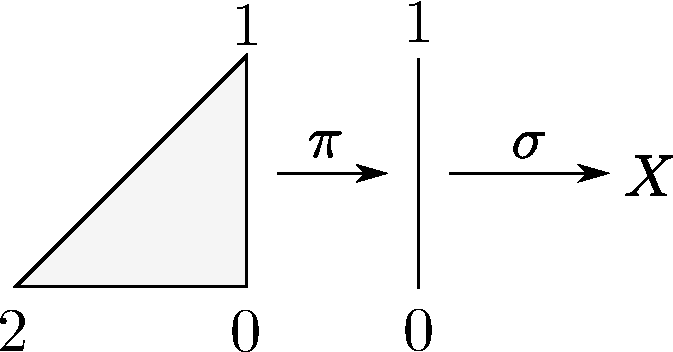
\includegraphics[width=3in]{905/Figures/02-projection.pdf}
\end{center}
 
We'll compute $d(\sigma\circ\pi)$. Some of the terms will be constant
singular simplicies. Let's write $c_x^n:\Delta^n\to X$ for the constant map 
with value $x\in X$. Then
\[
d(\sigma\circ\pi)=\sigma\pi d^0-\sigma\pi d^1 +\sigma\pi d^2=\overline{\sigma}-c^1_{\sigma(0)}+\sigma\,.
\]
The constant simplex $c^1_{\sigma(0)}$ is an error term, and we wish to 
eliminate it. To achieve this we can use the constant $2$-simplex $c^2_{\sigma(0)}$ at $\sigma(0)$; its boundary is
\[
c^1_{\sigma(0)}-c^1_{\sigma(0)}+c^1_{\sigma(0)}=c^1_{\sigma(0)}\,.
\] 
So 
\[
\overline{\sigma}+\sigma=d(\sigma\circ\pi + c^2_{\sigma(0)})\,,
\] 
and $\overline{\sigma}\equiv -\sigma\bmod B_1(X)$ as claimed.

Some more language: two cycles that differ by a boundary $dc$ are said to be {\em homologous}, and the chain $c$ is a {\em homology} between them. 

\end{example}

Let's compute the homology of the very simplest spaces, $\varnothing$ and $\ast$. For the first, $\Sin_n(\varnothing)=\varnothing$, so $S_\ast(\varnothing)=0$. Hence $\cdots\to S_2\to S_1\to S_0$ is the zero chain complex. This means that $Z_\ast(\varnothing)=B_\ast(\varnothing)=0$. The homology in all dimensions is therefore $0$.

For $\ast$, we have $\Sin_n(\ast)=\{c^n_\ast\}$ for all $n\geq 0$. Consequently $S_n(\ast)=\mathbf{Z}$ for $n\geq0$ and $0$ for $n\leq0$. 
For each $i$, $d_ic^n_\ast=c^{n-1}_\ast$, so
the boundary maps $d\colon S_n(\ast)\to S_{n-1}(\ast)$ in the chain complex depend on the parity of $n$ as follows:
\[d(c^n_\ast)=\sum_{i=0}^{n}(-1)^i c^{n-1}_\ast=
\begin{cases}
    c^{n-1}_* & \text{for } n \text{ even, and}\\
    0 & \text{for } n \text{ odd.}
  \end{cases}
\]
This means that our chain complex is:
\[
0\leftarrow0\leftarrow\ZZ\xleftarrow{1}\ZZ\xleftarrow{0}\ZZ\xleftarrow{1}\cdots\,.\]
The boundaries coincide with the cycles except in dimension zero, where $B_0(\ast)=0$ while $Z_0(\ast)=\mathbf{Z}$. Therefore $ H_0(\ast)=\mathbf{Z}$ and $ H_i(\ast)=0$ for $i\neq0$.

We've defined homology groups for each space, but haven't yet considered what happens to maps between spaces. A continuous map $f\colon X\to Y$ induces a map $f_\ast\colon \Sin_n(X)\to\Sin_n(Y)$ by composition: 
\[
f_\ast:\sigma\mapsto f\circ \sigma\,.
\] 
For $f_\ast$ to be a map of semi-simplicial sets, it needs to commute with face maps. Explicitly, we need $f_\ast \circ d_i = d_i \circ f_\ast$. A diagram is said to be \emph{commutative} if all composites with the same source and target are equal, so this equation is equivalent to commutativity of the diagram
\begin{eqnarray*}
\xymatrix{\Sin_n(X)\ar[r]^{f_\ast}\ar[d]^{d_i} & \Sin_n(Y)\ar[d]^{d_i}\\
\Sin_{n-1}(X)\ar[r]^{f_\ast} & \Sin_{n-1}(Y)\,.}
\end{eqnarray*}
We see that $d_if_\ast\sigma=(f_\ast\sigma)\circ d^i=f\circ\sigma\circ d^i$, and $f_\ast(d_i\sigma)=f_\ast(\sigma\circ d^i)=f\circ\sigma\circ d^i$ as desired. The diagram remains commutative when we pass to the free abelian groups of chains.

If $C_\ast$ and $D_\ast$ are chain complexes, a \emph{chain map} $f\colon C_\ast\to D_\ast$ is a collection of maps $f_n\colon C_n\to D_n$ such that the following diagram commutes for every $n$:
\begin{equation*}
    \xymatrix{
	C_n\ar[r]^{f_n}\ar[d]^{d_C} & D_n\ar[d]^{d_D}\\
	C_{n-1}\ar[r]^{f_{n-1}} & D_{n-1}
    }
\end{equation*}
For example, if $f\colon X\to Y$ is a continuous map, then $f_\ast \colon S_\ast(X)\to S_\ast(Y)$ is a chain map as discussed above.

A chain map induces a map in homology $f_\ast: H_n(C)\to H_n(D)$. The method of proof is a so-called ``diagram chase'' and it will be the first of many. We check that we get a map $Z_n(C)\to Z_n(D)$. Let $c\in Z_n(C)$, so that $d_C c = 0$. Then $d_D f_n(c) = f_{n-1}d_C c = f_{n-1}(0) = 0$, because $f$ is a chain map. This means that $f_n(c)$ is also an $n$-cycle, i.e., $f$ gives a map $Z_n(C)\to Z_n(D)$.

Similarly, we also get a map $B_n(C)\to B_n(D)$. Let $c\in B_n(C)$, so that there exists $c^\prime \in C_{n+1}$ such that $d_C c^\prime = c$. Then $f_n(c) = f_nd_C c^\prime = d_D f_{n+1}(c^\prime)$. Thus $f_n(c)$ is the boundary of $f_{n+1}(c^\prime)$, and $f$ gives a map $B_n(C)\to B_n(D)$.

The two maps $Z_n(C)\to Z_n(D)$ and $B_n(C)\to B_n(D)$ quotient to give a map on homology $f_\ast: H_n(X)\to H_n(Y)$, as desired.
